\section{A Two Agents Model}\label{sec:AgentModel}

All the models and strategies that we explore later in the experiments show similar features. This is due to the fact that each of these models and strategies derives from a unique model that features two agents. These two agents are defined by a set of functions that they both share, by some knowledge that they only partially share and by a set of states which they can go in, each state deciding the agents' actions during the argumentation.

The different models of argumentation on the meaning varies by the error management of the model's machine learning component. On the other hand, the different strategies of argumentation on the meaning varies by the set of states in which the agents can go in.

We qualify our model as symmetrical, since for a given model and strategy the set of functions of the agents is identical, the set of states of the agents is identical, and the knowledge shared by one agent is also shared by the other.

\subsection{Agent Knowledge}

While we are in the position of an oracle and have access to the entire knowledge of both agents, each agent has itself limited knowledge over the elements that are belonging to the other agent.

In order to clarify to which knowledge which agent has access to, we are classifying the agents' knowledge in three categories: \emph{personal} knowledge, \emph{overall} knowledge and \emph{inferred} knowledge.

The personal knowledge is only accessible to one agent $A_{k}$. The overall knowledge is accessible to both agents $A_{k}$ and $A_{-k}$. The inferred knowledge is a knowledge accessible to $A_{k}$ that is mirroring, with a varying degree of accuracy, a knowledge either only accessible to $A_{-k}$ or a knowledge accessible neither to $A_{k}$ or $A_{-k}$.

\subsubsection{Personal Knowledge}

An agent $A_{k}$ has access to a contrast set, called the initial contrast set $K^{0}_{k}$, and all the elements from this contrast set -- the contrast set's concepts and the semiotic elements from these concepts. Agents can also create new contrast sets. If an agent comes to create a new contrast set, called the \emph{current} contrast set $K_{k}$ by opposition to the initial one, this agent has also access to this contrast set. When we mention a contrast set without precision on whether it is the initial or current contrast set, it is by default the current contrast set.

\subsubsection{Overall Knowledge}

The overall knowledge is the knowledge that one agent shares, at least partially, with the other agent. This category of knowledge can be divided in two categories: the \emph{shared} knowledge that is directly shared with the other agent through messages, and the \emph{inferred} knowledge that is deduced from the other agent's knowledge without being directly exchanged by messages.

\paragraph{Shared Knowledge}

The shared knowledge is transmitted through messages. Since a message can only contain either semiotic elements or triplets, the shared knowledge is limited to some semiotic elements from both agents and their relations. Since exchanging messages has a cost, the agents try to reduce the amount of shared knowledge during an argumentation. The examples that an agent has sent or received are recalled in a specific set, noted $U_{ex}$. This set of example helps the agent to not exchange an example twice, and is used to infer additional knowledge. The generalizations, always exchanged by sets corresponding to intensional definitions, can be stored in an agent $A_{k}$'s hypothesis $H_{k}$ when they are received. The intensional definitions are always received with an associated sign. While the hypothesis of an agent contains concepts and not intensional definitions alone, only the intensional definitions of the hypotheses' concepts and their signs are shared by both agents. The extensional definitions from the hypotheses' concepts are only inferred by the agent. The triplets received are used to infer overall triplets and overall pairing relations, which is discussed in the \emph{inferred knowledge} paragraph.

\paragraph{Inferred Knowledge}

From the intensional definitions received by an agent, the other agent can infer an approximation of the other agent's concept associated extensional definition (see Section \ref{sec:funCreaConI}) by using its own adjunct set instead. This allows the agent to create a new concept that can be stored in its hypothesis, which represents the agent's guess on the concepts of the other agent. An agent can infer the overall relation between one of its concept and one of the other agent's concept as described in Section \ref{sec:Overall}. Once an overall pairing relation has been inferred, this agent can identify if this pairing relation induces a disagreement. If the paring relation is causing a disagreement, this disagreement is formalized into a triplet (see Section \ref{sec:SynD}) and recalled in a set of active disagreements $D$.

The distinction between personal knowledge and inferred knowledge is perfectly illustrated in the Section \ref{sec:Knowledge} with the beliefs and arguments. While an e-argument represents a knowledge that is known as a fact by an agent, a belief represents a knowledge that the agent has inferred but is partially unsure of. Personal knowledge is exchanged by an agent to attack the inaccurate parts of the inferred knowledge of another agent. On the other hand, shared knowledge is supposed to be known by both agents and therefore should not be exchanged at all.

\subsection{Agent Modus Operandi}
\label{sec:ModusOperandi}

The argumentation takes place turn by turn, with one agent receiving a token at the beginning of the argumentation, taking a set of actions, then passing the token to the other agent. An agent can take actions only when it has the token, and the last action that it takes is always to pass the token to the other agent. The token is exchanged until termination is detected. The actions taken by an agent while it has the token are decided by the agent's inputs and its current state. The two variables that impact the behaviour of one agent at a given turn are the agent's state (a qualitative variable) and the messages that this agent has received from the other agent. Each agent has the same set of possible states, making our argumentation model \emph{symmetric}.

The argumentation model is also synchronized, meaning that if an agent $A_{1}$ is in a state \#1 during the turn $t$, the agent $A_{2}$ was either in the state \#1 during the previous turn $t_{-1}$ or will be in the state \#1 during the next turn $t_{+1}$.

\subsection{Agent Functions}

\subsubsection{Inductive Learning}

\label{sec:funIndLearn}
The agents are inductive learners. Being able to use inductive learning over a set of examples in order to obtain a set of generalizations that subsume these examples without subsuming the rest of the subset is the most fundamental function of our agents. Each agent use the ABUI algorithm in order to achieve inductive learning. An agent $A$ with a local context $U_{k}$ needs to split its context in two subsets $E$ and $E'$ such that $E \cup E' = U_{k}$ and $E \cap E' = \emptyset$. Once these two sets of examples have been created and passed as inputs of ABUI, ABUI returns an intensional definition $I = \{g_{1}, \ldots, g_{n}\}$ such that:

\begin{itemize}
\item $\forall e \in E, \exists g \in I$ such that $g \sqsubseteq e$
\item $\forall e \in E', \nexists g \in I$ such that $g \sqsubseteq e$
\end{itemize}

The ABUI algorithm cannot always guarantee that the intensional definition returned verifies these two properties, but it approaches them as much as it can by minimizing the number of examples from $E'$ that are subsumed by $I$, and the number of examples from $E$ that are not subsumed by $I$. While the rest of this section does not take into account these errors of first and second order, their impact is discussed later in Section \ref{sec:DoGGenIdea}.

\subsubsection{Naming Examples}
\label{sec:funName}

The agents can name the examples presented to them. When an agent names an example $e$, it always uses a left-path associations to find $e$'s associated sign. The container used by the agent to name $e$ is its current contrast set $K$, or the initial contrast set if no current contrast set had been created by the agent. When naming an example $e$ with its contrast set $K$, an agent returns the set of signs $\{s_{1},...,s_{n}\}$ such that $e \prescript{l}{K}{\mapsto} \{s_{1},...,s_{n}\}$.

\subsubsection{Sending and Receiving Messages}
\label{sec:funMessages}

An agent can send a message to another agent. A message has two parts: a performative and a content.
The performative of the message indicates to the other agent the intent of the message, while the content vehicles a knowledge that the sender has.
The different types of messages are presented in Appendix \ref{apx:Messages} along with their associated performatives and contents.

When an agent sends a message, it arrives in the mailbox of the other agent. The message stays in the mailbox until the other agent removes it. In Section \ref{sec:ModusOperandi}, we mentioned that agents were taking actions turn by turn. These actions are mostly determined by the state of an agent during its turn, but also by the messages that are in the mailbox. It can happen that a message from an agent $A_{1}$ is not supposed to be read by an agent $A_{2}$ before $A_{2}$ is a certain state. For this reason, each message is timed for a defined state noted \#State. The message will only be delivered to the other agent when this agent enters the timed state for the next time.

For instance, in our model, the agents $A_{1}$ and $A_{2}$ goes through two states \#1 and \#2 where they respectively evaluate the local r-triplets of each other, and the overall r-triplets of each other. Let's assume that $A_{1}$ enters State \#1 first. It is supposed to have received (local) r-triplets from \emph{Evaluation} messages sent by $A_{2}$, and to compare these r-triplets with its own local r-triplets. Doing so allows $A_{1}$ to find the overall r-triplets, as explained in \ref{sec:Overall}. After this, $A_{1}$ sends the overall r-triplets that it just found to $A_{2}$ with an \emph{Evaluation} message, and passes the token to $A_{2}$. Upon receiving the token, $A_{2}$ enters State \#1 and follows the same instructions as $A_{1}$ did during the previous turn. However, additionally to the \emph{Evaluation} messages containing the local r-triplets from $A_{1}$ that any agent is supposed to have received at the beginning of State \#1, $A_{2}$ has also received the overall r-triplets sent by $A_{1}$ during the previous turn, and that are not needed until State \#2. Since both sets of messages carry the same performative and the same type of content, $A_{2}$ does not know which r-triplet it is supposed to consider as local r-triplets to compute the overall r-triplets, and which r-triplets it is supposed to ignored. Timing the \emph{Evaluation} messages sent by $A_{1}$ during State \#1 in order for them to be received by $A_{2}$ only when $A_{2}$ enters State \#2 solves this issue.

The notation of a message is the following; a message with:

\begin{itemize}
    \item a performative \emph{Performative},
    \item a content $T = \{ T_{1}, \ldots, T_{}n \}$ were each $T_{i}$ is a different type of content, and
    \item timed for the agent state \#State
\end{itemize}

is noted \emph{Performative}\#State($T_{1}$, $\ldots$, $T_{n}$)

\subsubsection{Computing Adjunct Sets}
\label{sec:funCompAdj}

After naming examples, the most basic function that an agent should have is to compute adjunct sets of concepts. This function links the left-path and the right-path associations by retrieving the set of examples subsumed by the intensional definition of a concept. By default, the adjunct set is computed using the current contrast set of the agent. The notion of adjunct set is defined in Definition \ref{def:AdjC}. An agent $A_{k}$ computes the adjunct set of a concept $C = \langle s, I, E \rangle$ such that $I = \{g_{1}, \ldots, g_{n}\}$ by directly creating the set of examples $Adj(C,U_{k}) = \{ e \in U_{k} | \exists g \in I \wedge g \sqsubseteq e \}$.

\subsubsection{Computing Local R-Triplet and Pairing Relation}
\label{sec:funCompRT}

Using its adjunct sets, an agent $A_{k}$ can find the local pairing relation between two concepts $C_{i}$ and $C_{j}$ as explained in Section \ref{sec:Adj&Relations}. First, $A_{k}$ builds the local r-triplet $r(C_{i}, C_{j}, U_{k})$, and then computes the local pairing relation $r_{Uk}$ using Definition \ref{def:Relation}.

\subsubsection{Inferring Overall Pairing Relation from Received Triplets}
\label{sec:funInferOv}

Using the composition law presented in Theorem \ref{thm:Overall}, an agent can infer an overall pairing relation between two concepts $C_{i}$ and $C_{j}$ from a local pairing relation received from another agent and its own corresponding local pairing relation. However, the two agents need the intensional definitions of both $C_{i}$ and $C_{j}$ in order to compute their local r-triplets and infer the overall pairing relation. Once the overall relation of two concepts is obtained, the agents know if these two concepts are causing a semantic or lexical disagreement. 

In a model using Boolean r-triplets, having both local triplets is enough to find the overall relation between two concepts from different agents. However, in a model that admits a degree of error and uses integer r-triplets, the agents might need to exchange more knowledge. This problem is discussed in Section \ref{sec:DoGGenIdea}.

\subsubsection{Disagreement Listing}
\label{sec:funListD}

Finding and listing the disagreements in order to resolve them is one of the main functions of the agents. In order to resolve a disagreement, both agents should be aware of its existence and have characterized it: they should know which signs and pairing relation (or absence of relation) is behind it. That is why the disagreements are always characterized in the overall context. Before starting to resolve their disagreements, the agents should exchange enough knowledge to be certain of the nature of the eventual overall relations that cause these disagreements.

As soon as two local relations involving the two same concepts are exchanged, the agents can categorize and list the semantic, lexical or self disagreements depending on the inferred overall relation and origin of the two concepts. An untranslatable disagreement, on the other hand can only be listed to an extensive transfer of the agents' intensional definitions and the inference of all the overall pairing relations, as it is characterized by the \emph{absence} of a pairing relation.

In the case of the lazy strategy presented in Chapter \ref{LazyStrategy}, the agents do not exchange all their intensional definitions at the start of the argumentation, and therefore have to be vigilant on the fact that each concept belonging to a same system of disagreement should have an equivalent in another contrast-set.

\subsubsection{Creating New Signs}
\label{sec:funCreaSign}

Each agent can create a sign. The creation of a new sign is simple, as the signs are in an arbitrary relation with the two other semiotic elements. The created signs are ensured to be all different by keeping track of the previously created signs, and by choosing a specific structure for the new signs that differentiates them from the signs that are already existing in the agents' contrast sets. For instance, in our implementation, all the new signs start with the radical \emph{newSign\_}, followed by a unique number that is incremented each time that a sign is created.

The sign created by an agent can also be used by another agent, as long as this sign has been sent to the other agent along with the semiotic element to which it is associated.

\subsubsection{Creating New Concepts from Right-Path Associations}
\label{sec:funCreaConE}

\begin{figure}[t]
    \centering
    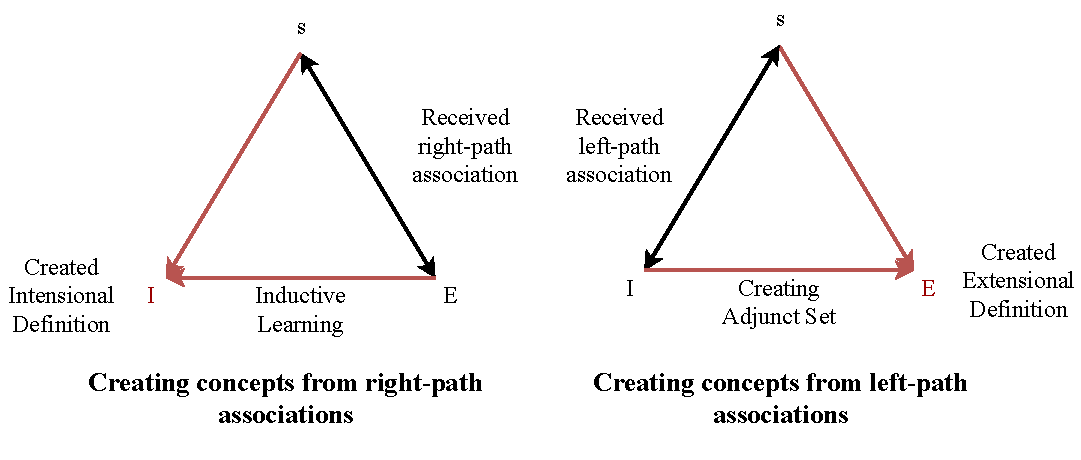
\includegraphics[width=\textwidth]{figs/ConceptCreation.pdf}
    \caption{The creation of a concept $C = \langle s,I,E \rangle$ from a right-path association (left) and a left-path association (right), by respectively retrieving the intensional definition through inductive learning and retrieving the extensional definition through the computation of the adjunct set.}
    \label{fig:ConCrea}
\end{figure}

An agent can learn a new concept if it received a set of examples associated to one sign. If the agent receives the class $U(\mapsto s)$, it can learn by inductive learning a new intensional definition $I = \{g_{1}, \ldots, g_{n}\}$ such that $I$ subsumes $U$. Other classes can be involved in the learning as negative examples: for instance, if an agent receives two classes $U_{+}(\mapsto +)$ and $U_{-}(\mapsto -)$ and wishes to create a concept that corresponds to the first class, it can learn an intensional definition $I_{+}$ that covers the examples $U_{+}$ without covering the examples $U_{-}$.

In our model, these intensional definitions are learned through inductive learning, using the ABUI algorithm. Any machine learning technique can be used to create a set of generalizations that respect these properties (only subsuming the examples from the designed class). However, in the case where an absolutely accurate learning is not guaranteed or possible, the model needs to be adapted to account a certain degree of error. The aforementioned adaptations are presented in Section \ref{sec:DoGGenIdea}.

Once the agent has created an intensional definition $I$, it creates the new concept $C = \langle s,I,U_{+} \rangle$ as the association of the three semiotic elements. Agents mostly create concepts in this fashion to create their initial contrast sets, when they receive their initial sets of right-path associations. They also use this method to generate new beliefs, when they need to cooperatively create new concepts with other agents without having an intensional definition upon which to base this creation. 

\subsubsection{Creating New Concepts from Left-Path Associations}
\label{sec:funCreaConI}

When an agent does not directly have access to the right-path associations, it can still create a concept from an intensional definition $I$ and a sign $s$ by creating the adjunct set of the concept from which $I$ and $s$ originates, as the adjunct set only requires an intensional definition to be computed. By doing so, the agent obtains a set of left-path associations. If an agent $A_{k}$ receives an association $I = \{g_{1}, \ldots, g_{n}\} \mapsto s$, it can directly create the concept $C = \langle s, I,  Adj(I,U_{k}) \rangle$.

\subsubsection{Creating New Concepts through Argumentation}
\label{sec:funCreaConA}

\begin{figure}[t]
    \centering
    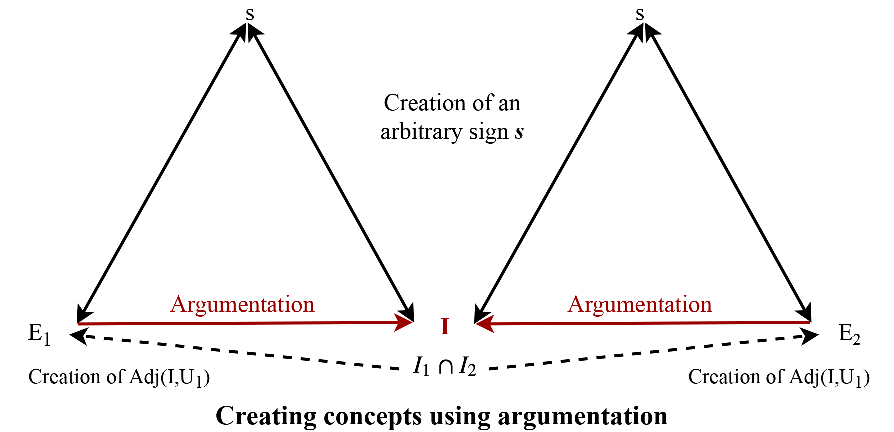
\includegraphics[width=0.78\textwidth]{figs/CoopConceptCreation.pdf}
    \caption{The creation of a new concept through the use of argumentation. The main steps are: determining an overall pairing partial sets from two intensional definitions, creating the corresponding local partial sets, arguing on the adequacy of proposed intensional definitions for the overall pairing partial set, and creating an arbitrary sign.}
    \label{fig:CoopConCrea}
\end{figure}

Creating a new concept $C_{n} = \langle s_{n}, I_{n}, E_{n} \rangle$ using either left or right-path associations requires for the agent to have at least two of $C_{n}$'s semiotic elements -- its sign and either its extensional or intensional definition. However, our model requires the agents to create new concepts which they have no semiotic element of, in order to resolve several types of disagreements. In situations like these, the agents can only create a new concept by arguing with each others.
% Define the extensional definition in the overall context

First, the two agents need to determine which subset of the overall context will be the extensional definition of a new concept. This set is noted $U_{n}^{+} = Adj(C_{n},U_{O})$, as the extensional definition of our new concept $C_{n}$ should ideally be $C_{n}$'s adjunct set according to Definition \ref{def:AdjC}.
% Cannot access the overall context, so need to decide using intensional definitions
In the context of a disagreement which involves two concepts $C_{1}$ and $C_{2}$, $U^{+}_{n}$ is determined to be one of the overall pairing partial sets $U_{O,1,\overbar{2}}, U_{O,1,2}, U_{O,\overbar{1},2}$ of $C_{1}$ and $C_{2}$. The choice of a particular set depends on the type disagreement that the agents are resolving, which we discuss later in Section \ref{sec:Resolution}.

% Positive and negative sets of examples are consistent
The relative complement of $U^{+}_{n}$ with respect to $U_{O}$ is noted $U^{-}_{n}$. Together, $U^{+}_{n}$ and $U^{-}_{n}$ partition the overall context $U_{O}$. Even if it has determined which overall pairing partial set of the pair of concept $C_{1},C_{2}$ is $U^{+}_{n}$, $A_{k}$ cannot directly access the sets $U^{+}_{n}$ and $U^{-}_{n}$ as it might contains examples from $U_{-k}$. $A_{k}$ can only access its local examples of $U^{+}_{n}$, the set $U^{+}_{n,k} = U^{+}_{n} \cap U_{k}$.

% Create a sign
The next step for the agents is to create an arbitrary sign $s_{n}$ that each agent $A_{k}$ will associate with its set of examples $U^{+}_{n,k}$. Since $s_{n}$ only has the requirement of not belonging to the agents' joint vocabulary, any agent can create $s_{n}$ and send it to the other agent. Once both agents have associated their sets of examples $U^{+}_{n,k}$ with the sign $s_{n}$, they each have a set of association $U^{+}_{n,k} \prescript{r}{k}{\mapsto} s_{n}$. One agent $A_{1}$ is then chosen to create a new intensional definition from this set of right-path associations, using the same method as for the creation of new concepts using right-path associations detailed in Section \ref{sec:funCreaConE}. $A_{1}$ is chosen accordingly to the type of disagreement that $C_{n}$ is supposed to help resolving, which we discuss later in Section \ref{sec:Resolution}.

% Change the intensional definition
Since $U^{+}_{n,1}$ is only a subset of $U^{+}_{n}$, there is an important risk that the intensional definition $I^{t1}_{1}$ which is
learned over $U^{+}_{n,1}$ subsumes examples subsumes examples that belong to the set $U^{-}_{n,2} = U^{-}_{n} \cap U_{2}$, or on the contrary does \emph{not} subsume examples from $U^{+}_{n,2}$. Since $U^{+}_{n,2}$ and $U^{-}_{n,2}$ are also subsets of respectively $U^{+}_{n}$ and $U^{-}_{n}$, a such scenario would imply that $I^{t}_{n}$ is not fit to be the extensional definition of $U^{+}_{n}$. In order to help $A_{1}$ to create a suitable intensional definition for $U^{+}_{n}$, the agent $A_{2}$ can argue about the fitness of $I^{t1}_{n}$ over $U^{+}_{n}$ so $A_{1}$ can create a more fitting intensional definition $I^{t2}_{n}$. This argumentation can be done over any intensional definition $I^{tx}_{n}$ until a final intensional definition $I^{tF}_{n}$ that is suitable for $U^{+}_{n}$ is found. The argumentation framework used to find $I^{tF}_{n}$ is discussed in Section \ref{sec:funLeadArg}.
% Creating the concept(s)
Once the intensional definition is found, each agent $A_{k}$ creates its own version of the new concept $C^{k}_{n} = \langle s_{n}, I^{tF}_{n}, U^{+}_{n,k} \rangle$. Then, $A_{1}$ adds $C^{1}_{n}$ to its contrast set while $A_{2}$ adds $C^{2}_{n}$ to its hypothesis.

\subsubsection{Managing the Creation of a New Intensional Definition}
\label{sec:funLeadArg}

As mentioned in the previous section, only one agent is in charge of a new concept's creation through argumentation while the other agent is helping by arguing over the correctness of the relation between the new concept's extensional and intensional definitions. When an agent learns that it will have to create a new concept through argumentation, it decides whether or not to take the lead according to the following rules. The agent decides to take the lead if:

\begin{enumerate}
    \item it is the only one to have examples from the positive set of examples in its context \textbf{or}
    \item it has not received a message from the other agent indicating that the other agent took the lead \textbf{and}
    \item it has examples from the positive set of examples \textbf{and}
    \item it has the right container, decided upon the type of disagreement leading to the creation of a new concept.
\end{enumerate}

When an agent takes the leadership in the creation of the new intensional definition, it immediately sends a message to the other agent indicating so.

\section{Argumentation in Concept Creation}
\label{sec:Knowledge}

\subsection{Arguments as Binary Classifications}

% Explain why we need an argumentation
Before arguing in the process of a new concept $C_{n}$'s creation, the agents have already determined the extensional definition and the sign of the new concept. The agents are however missing the intensional definition $I(C_{n})$k, and the argumentation is what will help them to find it. As we mentioned in Section \ref{sec:funCreaConA}, the main issue with finding $I(C_{n})$ is that the agents need to ensure that $I(C_{n})$ is subsuming every elements of $U^{+}_{n}$ without subsuming any element of $U^{-}_{n}$. This requires to test all the elements of the overall context, which cannot be done by one agent individually as none of the agents is supposed to have access to the overall context.

% Explain the binary classification
The agents can however overcome this issue by cooperating in the creation of $I(C_{n})$. In order to explain how, let's consider the creation of $I(C_{n})$ as a binary classification over $U_{O}$. The agents want $I(C_{n})$ to subsume the examples of the extensional definition $U^{+}_{n}$ without subsuming the other examples from $U_{O}$, $U^{+}_{n}$ is similar to a set of positive elements. Likewise, the set of examples $U^{-}_{n}$ is similar to a set of negative elements since it is the relative complement of $U^{+}_{n}$ with regard to the entire population of our test $U_{O}$. By subsuming or not the examples of $U_{O}$, $I(C_{n})$ creates another partition of $U_{O}$ into positive and negative assignments. The positive assignments of $I(C_{n})$ are the examples $\{e \in U_{O} | I(C_{n}) \sqsubseteq e \}$, which according to Definition \ref{def:AdjI} is the adjunct set of $I(C_{n})$. The set of negative assignments of $I(C_{n})$ is $\{e \in U_{O} | I(C_{n}) \not \sqsubseteq e \}$, equivalent $U_{O} - Adj(I(C_{n}),U_{O})$. In order to be an intensional definition for $C_{n}$.

% Can measure the adequateness of any intensional definition
According to Definition \ref{def:Con}, $I(C_{n})$'s set of positive assignments should be equivalent to the set of positive elements in order for $I(C_{n})$ to be an adequate intensional definition for $C_{n}$. Representing $I(C_{n})$ as a binary classification allows us to measure the adequacy of any intensional definition $I$ to the role of intensional definition of $C_{n}$ in terms of true positives, true negatives, false positives and false negatives. These four sets are defined as:

\begin{itemize}
    \item The set of true positives of $I$ is $TP(I) = \{ e \in U^{+}_{n} | I \sqsubseteq e \}$
    \item The set of true negatives of $I$ is $TN(I) = \{ e \in U^{-}_{n} | I \not \sqsubseteq e \}$
    \item The set of false positives of $I$ is $FP(I) = \{ e \in U^{-}_{n} | I \sqsubseteq e \}$
    \item The set of false negatives of $I$ is $FN(I) = \{ e \in U^{+}_{n} | I \not \sqsubseteq e \}$
\end{itemize}

% Why we need an argumentation framework
If the intensional definition has $I$ no false positives or false negatives, therefore the set of $I$'s positive assignments is equivalent to the set of positive elements and $I$ is suitable to be the intensional definition $I(C_{n})$ of the new concept $C_{n}$. Therefore, in order to be sure that $I = I(C_{n})$, the agents should agree that:

\begin{itemize}
    \item The set $FP(I) = \emptyset$
    \item The set $FN(I) = \emptyset$
\end{itemize}

As we mentioned, no agent has individually entirely access to $U^{+}_{n}$ or $U^{-}_{n}$. However, we know that the overall context is the union of the two local contexts, which means that:

\begin{itemize}
    \item $U^{+}_{n} = U^{+}_{n,1} \cup U^{+}_{n,2}$
    \item $U^{+}_{n} = U^{-}_{n,1} \cup U^{-}_{n,2}$
\end{itemize}

Therefore, the agents know that:

\begin{itemize}
    \item $U^{+}_{n,1} \cap U^{+}_{n,2} = \emptyset \Leftrightarrow U^{+}_{n} = \emptyset$
    \item $U^{-}_{n,1} \cap U^{-}_{n,2} = \emptyset \Leftrightarrow U^{-}_{n} = \emptyset$
\end{itemize}

While the agents cannot directly access $U^{+}_{n}$ and $U^{-}_{n}$, they can both locally verify that they have no knowledge of false positives or negatives and share this information in order to know if an intensional definition is suitable to be the intensional definition of $C_{n}$. Exchanging false positives and negatives is akin to an argumentation process.

% Basis of argumentation frameworks
An argumentation framework consists of a combination of a set of elements $A$ called \emph{arguments}, and a binary relation on $A$ called \emph{attack} relation. An argument $\gamma$ attacking another argument $\alpha$ is noted $\gamma \twoheadrightarrow \alpha$. An argument $\alpha$ represents a binary classification of the overall context $U_{0}$, partitioning $U_{O}$ into positive and negative assignments. Moreover, $\alpha$ should clarify which classification it intends to predict. The notion of argument is formally defined below in Definition \ref{def:Arg}:

\begin{restatable}[Argument]{df}{Argument}
\label{def:Arg}

Let $A_{1}$ and $A_{2}$ be two agents with an overall context $U_{O}$. The context $U_{O}$ is partitioned in two sets of examples $U^{a}$ and $U^{b}$. Let $a$ and $b$ be two signs such that $U^{a} \prescript{}{k}{\mapsto} a$ and $U^{b} \prescript{}{k}{\mapsto} b$ for all agents $A_{k}$. An argument $\alpha$ is a pair $(a,A_{k})$ that has an adjunct set $Adj(\alpha,U_{k}) = U^{a} \cap U_{k}$. Conceptually, the adjunct set of $\alpha$ is a binary classification function such that:

\begin{itemize}
    \item $U^{a}$ is the set of positive elements of $\alpha$
    \item $U^{b}$ is the set of negative elements of $\alpha$
    \item $Adj(\alpha,U_{O})$ is the set of positive assignments of $\alpha$
    \item $U_{O} - Adj(\alpha,U_{O})$ is the set of negative assignments of $\alpha$
\end{itemize}

and represents the fact that:

\begin{itemize}
    \item $A_{k}$ \textbf{knows} that $Adj(\alpha,U_{k}) = U^{a} \cap U_{k}$
    \item $A_{k}$ \textbf{expects} that $Adj(\alpha,U_{O}) = U^{a}$
\end{itemize}

\end{restatable}

During the process of creating a new concept, the aim of the argumentation between our agents is to generate an argument which extension is the set of examples $U^{+}_{n}$. A such argument proves that the agent that created it has enough knowledge over the overall context to generate an intensional definition suitable for the new concept.

\subsection{Evaluating Arguments}

In our argumentation framework, arguments are sorted into \emph{accepted} and \emph{rejected} arguments according to the following marking function:

\begin{itemize}
    \item an argument $\alpha$ is \emph{accepted} if none of the arguments attacking $\alpha$ is accepted, and
    \item an argument $\alpha$ \emph{rejected} if at least one of the arguments attacking $\alpha$ is accepted
\end{itemize}

Our argumentation framework is generative, meaning that instead of having a set of arguments and attacks before hand over which we apply a label function that determines which of these arguments are accepted, an agent $A_{k}$ can decide whether or not an argument $\alpha$ from the other agent should be acceptable in the first place. If $\alpha$ should not be acceptable and yet is accepted, $A_{k}$ can generate another argument $\gamma$ such that $\gamma \twoheadrightarrow \alpha$. The argument $\alpha$ being attacked makes it automatically defeated.

In order to determine whether or not an argument $\alpha$ is acceptable, an agent $A_{k}$ searches for false positives and negatives. According to Definition \ref{def:Arg}, we can write the false positives and false negatives of the argument $\alpha$ as follow:

\begin{itemize}
    \item \textbf{FP($\alpha$)} = $U^{b} \cap Adj(\alpha,U_{O})$
    \item \textbf{FN($\alpha$)} = $U^{a} \cap (U_{O} - Adj(\alpha,U_{O}))$
\end{itemize}

From the expression of false positives and negatives of $\alpha$, we can infer a group of properties that are useful to determine how the argument $\alpha$ should be considered as acceptable by $A_{k}$.

\begin{restatable}{pp}{FPalpha}
\label{pp:FPalpha}
Let $A_{1}$ and $A_{2}$ be two agents with an overall context $U_{O}$. Let $U_{O}$ be partitioned in two sets of examples $U^{a}$ and $U^{b}$, and let $\alpha = (a,A_{-k})$ be an argument of $A_{-k}$. The set of $\alpha$'s false positives in $U_{k}$ is empty if and only if FP($\alpha$) is empty.

\end{restatable}

\begin{restatable}{pp}{FNalpha}
\label{pp:FNalpha}
Let $A_{1}$ and $A_{2}$ be two agents that have their overall context $U_{O}$ partitioned in two sets of examples $U^{a}$ and $U^{b}$, and let $\alpha = (a,A_{-k})$ be an argument of $A_{-k}$. The set of $\alpha$'s false negatives in $U_{k}$ is empty if and only if FN($\alpha$) is empty.

\end{restatable}

\begin{restatable}{pp}{Adequacy}
\label{pp:FNFPaccept}

Let $A_{1}$ and $A_{2}$ be two agents that have their overall context $U_{O}$ partitioned in two sets of examples $U^{a}$ and $U^{b}$, and let $\alpha = (a,A_{-k})$ be an argument of $A_{-k}$. If the set of $\alpha$'s false positives and $\alpha$'s false negatives in $U_{k}$ are both empty, then $Adj(\alpha,U_{O}) = U^{a}$.

\end{restatable}

\subsubsection{Counter-Argument}

% If both FP(alpha) and FN(alpha) are empty, then expectations of A_{-k} were right and alpha should be accepted
Property \ref{pp:FNFPaccept} states that if both FP($\alpha$) and FN($\alpha$) are empty, then the expectations of $A_{-k}$ were right as $Adj(\alpha,U_{O}) = U^{a}$. This means that if $A_{k}$ does not find false positives or negatives of $\alpha$ in its local context, then $A_{k}$ should accept the argument $\alpha$.
% Otherwise, send an argument to A_{-k} to inform that there are true/false positives.
Otherwise, $A_{k}$ should generate another argument $\gamma$ for each set of $FP(\alpha), FN(\alpha)$ which is non empty, such that $\gamma \twoheadrightarrow \alpha$. We say that $\gamma$ is a counter-argument. The notion of counter argument is defined below in Definition \ref{def:CArg} :

\begin{restatable}[Counter-Argument]{df}{CArgument}
\label{def:CArg}

Let $A_{1}$ and $A_{2}$ be two agents that have their overall context $U_{O}$ partitioned in two sets of examples $U^{a}$ and $U^{b}$, and let $\alpha = (a,A_{-k})$ be an argument of $A_{-k}$. The argument $\gamma = (x,A_{k})$ of $A_{k}$ is a counter argument  such that $\gamma \twoheadrightarrow \alpha$ if:

\begin{itemize}
    \item $Adj(\gamma,U_{k}) = FN(\alpha)$, if $x = a$
    \item $Adj(\gamma,U_{k}) = FP(\alpha)$, if $x = b$
\end{itemize}

\end{restatable}

The definition of counter arguments makes them arguments, implying that counter arguments can be attacked by other counter arguments, building up a tree that we call the argumentation tree.

\subsubsection{Accepted vs. Agreed Upon}

Each argument in the argumentation tree is either accepted or rejected. The function that marks the arguments as accepted and rejected is called the marking function. Each time that a new argument appears in the argumentation tree, the marking of the arguments change. There is a difference between an argument $\alpha = (a,A_{k})$ that is accepted because $A_{-k}$ did not have the opportunity to generate an attack against $\alpha$ yet, and an argument $\alpha'$ that has been considered acceptable by $A_{-k}$. In the former case, the marking of $\alpha$ as accepted can be temporary, while an argument $\alpha' = (a,A_{k})$ that has been deemed acceptable by $A_{-k}$ will remained accepted. This difference is marked by the conceptual distinction between \emph{accepted} arguments, that are just temporary marked as accepted, and arguments \emph{agreed upon}, that are definitively marked as accepted.

\subsection{Root Arguments}

\begin{figure}[t]
    \centering
    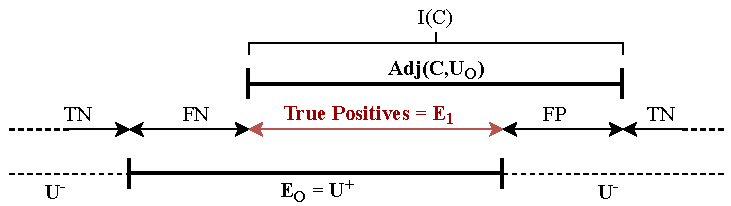
\includegraphics[width=\textwidth]{figs/Belief.pdf}
    \caption{The examples subsumed by an intensional definition $I(C)$ (top bracket) might be different from the examples that $I(C)$ is intended to subsume, especially if $I(C)$ was created without access to some of these examples. These differences are either false positives for the examples subsumed by $I(C)$ that were not intended to be, and false negative for the examples that are not subsumed by $I(C)$ but were intended to.}
    \label{fig:Belief}
\end{figure}

In order to find if an intensional definition $I$ is suitable to be the intensional definition of the new concept, $I$ will be transformed into an argument and the agents will be attacking it. In order to transform any intensional $I$ definition into an argument $\alpha$, $I$ needs to be associated to a sign $s \in \{+,-\}$. The sign $s$ determines which set from $U^{+}_{n}$ and $U^{-}_{n}$ should be the set of positive elements in the binary classification. If $I$ is a candidate for the intensional definition of $C_{n}$, then $s = +$. If this is the case, $I$ is said to be a \emph{root} argument. An argument is always associated to an agents $A_{k}$ that creates it. In the case of a root argument, this agent is the agent that leads the creation of the new concept. Root arguments are defined below in Definition \ref{def:RArg}:

\begin{restatable}[Root Argument]{df}{RArgument}
\label{def:RArg}

Let $A_{1}$ and $A_{2}$ be two agents, let $I = \{ g_{1}, ..., g_{m} \}$ be a set of generalizations and  $U_{O}$ the overall context of the agents, divided in two sets of examples $U^{+}$ and $U^{-}$ that partition the overall context. A root argument $\alpha = (+,I,A_{k})$ means that:

\begin{itemize}
    \item $A_{k}$ \textbf{knows} that $I \sqsubseteq U^{+}_{n,k}$ and $\nexists e \in U^{-}_{n,k}$ such that $I \sqsubseteq e$.
    \item $A_{k}$ \textbf{expects} that $I \sqsubseteq U^{+}_{n}$ while $\nexists e \in U^{-}_{n}$ such that $I \sqsubseteq e$.
\end{itemize}

\end{restatable}

\subsubsection{Generating Root Arguments}

The set of generalization $I$ of a root argument should subsume the examples of $U^{+}_{k}$ without subsuming the examples from $U^{-}_{k}$. The task of creating $I$ is given to the ABUI algorithm. The ABUI algorithm takes two classes, $U(\mapsto a)$ and $U(\mapsto b)$, and a sign $s \in \{a, b\}$. The ABUI algorithm returns a set of generalizations $I$ that subsumes all the examples from the class $U(\mapsto s)$ without subsuming any example from the other class $U(\mapsto S-s)$. In order to obtain $I$, the ABUI algorithm is given the two classes $U^{+}_{n,k}$ and $U^{-}_{n,k}$, with the sign $+$.

The ABUI can take an additional parameter, a set of generalization-sign associations $AA = G \mapsto S$, where $G$ is a set of generalizations $\{g_{1}, \ldots, g_{j} \}$ and $S$ is the lexicon $\{ a, b \}$. While looking for a suitable set of generalizations $I = g'_{1}, \ldots, g'_{p} $ that subsumes the examples of $U(\mapsto a)$ without subsuming the examples of $U(\mapsto b)$, ABUI ensures that:

\begin{itemize}
    \item for each generalization-sign association $g \mapsto a \in AA$, there exists another generalization $g' \in I$ such that $g' \sqsubseteq g$.
    \item for each generalization-sign association $g \mapsto b \in AA$, there are no generalization $g' \in I$ such that  $g' \sqsubseteq g$.
\end{itemize}

By adding generalizations that subsumes the false positives or negatives of different arguments in $AA$, the agents decrease the chances of having ABUI outputting a generalization that subsumes false positives, while increasing the chances of outputting a generalization that subsumes false negatives. The ABUI algorithm might not find a satisfying set of generalizations for a root argument each time. An unsuccessful root argument creation translates into an empty intensional definition for the new concept and the argumentation stops immediately.

\subsubsection{Agreed Upon Root Arguments}

If a root argument $\alpha = (+,I,A_{k})$ is agreed upon, then $I$ is considered as accepted as the intensional definition of the new concept $C_{n}$. The agents have determined the three semiotic elements of $C_{n}$, and the creation of $C_{n}$ can be achieved. The argumentation in the context of the creation of $C_{n}$ can therefore stop. This is one of the two stopping condition of the argumentation on the creation of $C_{n}$, along with the generation of a root-argument with an empty intensional definition. 
 
\subsubsection{Rejected Root Arguments}

If a root argument $\alpha = (+,I,A_{k})$ created by $A_{k}$ is rejected, $A_{k}$ has two options. The argument $\alpha$ being rejected means that there are one or several counter-arguments $CA = \{\gamma_{1}, \ldots, \gamma_{m}\}$ attacking $\alpha$ that are accepted. The first option of $A_{k}$ is to generate $m$ counter-arguments that will attack all the arguments from $CA$, since $\alpha$ is rejected only if there is at least an argument from $CA$ that is not rejected.

Of course, this option is only available to $A_{k}$ if the arguments from $CA$ are not acceptable. If at least one of the arguments from $CA$ is acceptable and has been agreed upon, then $A_{k}$ needs to create another root argument in order to continue the argumentation. The improvement of the new proposed intensional definition over the intensional definition that has been rejected as a root argument, is the result of the set of generalization-sign $AA$ that increases in size during the argumentation.

\subsection{G-Arguments}
\label{sec:GArg}

\begin{figure}
    \centering
    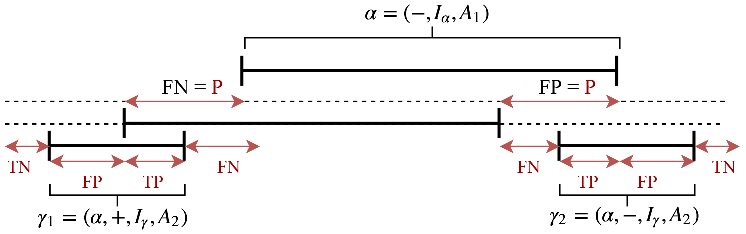
\includegraphics[width=\textwidth]{figs/Attack.pdf}
    \caption{As a belief, the intensional definition of a g-argument $\gamma$ intents to subsume the examples of a defined set (the false positives in the case of $\gamma_{1}$ or the false negatives in $\gamma_{2}$, of the belief $_{\alpha}$ that it attacks). Therefore, it also admits its own sets of false positives and false negatives, that can be attacked by other arguments themselves.}
    \label{fig:Attack}
\end{figure}

The root arguments are not the only class of arguments. The most similar class of argument to the root argument is the g-argument. Akin to the root arguments, the g-arguments are using an intensional definition to define their adjunct sets. However, since the g-arguments are not root arguments, they are always attacking another arguments and therefore are always counter arguments. The notion of g-argument is defined below in Definition \ref{def:GArg}:

\begin{restatable}[G-Argument]{df}{GArgument}
\label{def:GArg}

Let $A_{1}$ and $A_{2}$ be two agents that have their overall context $U_{O}$ partitioned in two sets of examples $U^{a}$ and $U^{b}$, and let $\alpha = (a,A_{-k})$ be an argument of $A_{-k}$. The g-argument $\gamma = (x,I,A_{k})$ is a counter argument of $A_{k}$ such that: 

\begin{itemize}
    \item for any context $U$, $Adj(\gamma,U) = Adj(I,U)$ and
    \item $Adj(I,U_{k}) = FN(\alpha)$, if $x = a$ or
    \item $Adj(I,U_{k}) = FP(\alpha)$, if $x = b$ or
\end{itemize}

\end{restatable}

\subsubsection{Accepted G-Arguments}

Every time that a g-argument gets accepted, the sets of accepted and rejected arguments of the argumentation tree are updated. If a g-argument $\gamma = (x,I,A_{k})$ stays accepted after the agent $A_{-k}$ had the opportunity to add a counter argument to the argumentation tree, the association $\gamma \mapsto x$ is added to the parameter $AA$ of the ABUI algorithm for the rest of the argumentation over the creation of $C_{n}$. 

\subsubsection{Rejected G-Arguments}

A rejected g-argument $\gamma$ stays in the argumentation tree. Every time that a g-argument gets rejected, the sets of accepted and rejected arguments of the argumentation tree are updated, as the argument $\alpha$ that $\gamma$ was attacking might now be accepted.

\subsection{E-Arguments}

The last class of arguments is the e-argument. An e-argument, unlike root arguments and g-arguments, does not use an intensional definition to define their adjunct sets, but rather uses directly a set of examples $E$. Since this set of example might not be a subset of the context of the agent that did not create the e-argument, the set of example $E$ is always set through an \emph{Examples} message along with the e-argument itself. Like to the g-arguments, e-arguments are counter arguments. The notion of e-argument is defined below in Definition \ref{def:EArg}:

\begin{restatable}[E-Argument]{df}{EArgument}
\label{def:EArg}

Let $A_{1}$ and $A_{2}$ be two agents that have their overall context $U_{O}$ partitioned in two sets of examples $U^{a}$ and $U^{b}$, and let $\alpha = (a,A_{-k})$ be an argument of $A_{-k}$. The g-argument $\gamma = (x,E,A_{k})$ is a counter argument of $A_{k}$ such that: 

\begin{itemize}
    \item for any context $U$, $Adj(\gamma,U) = E$ and
    \item $E = FN(\alpha)$, if $x = a$ or
    \item $E = FP(\alpha)$, if $x = b$ or
\end{itemize}

\end{restatable}

Since e-arguments require to exchange examples with other agents, they are not the privileged option during the generation of a counter argument and an agent that rejects an argument will always prefer to create an attack with a g-argument, in order to limit the example transfers between the agents.

\subsubsection{Accepted E-Arguments}

When an e-argument $\gamma = (x,E,A_{k})$ is accepted, its set of examples $E$ is added to the context of the agent $A_{-k}$. Since the acceptability of a g-argument and a root argument are always linked to the adjunct set and therefore to the context of an agent, changing the context of $A_{-k}$ always impact which arguments are deemed acceptable by $A_{-k}$. Moreover, every time that an e-argument gets accepted, the sets of accepted and rejected arguments of the argumentation tree are updated.

\subsubsection{Rejected E-Arguments}

An e-argument $\gamma = (x,E,A_{k})$ attacking an argument $\alpha = (a,A_{-k})$ cannot be attacked. Indeed, its adjunct set is its set of positive elements. Its adjunct set being its positive assignment, the set of positive assignments of $\gamma$ is therefore its set of positive elements and there cannot be false positives or negatives of $\gamma$. For this reason, e-arguments are always leaves on the argumentation tree.

\subsection{Argumentation Tree}

\begin{figure}
    \centering
    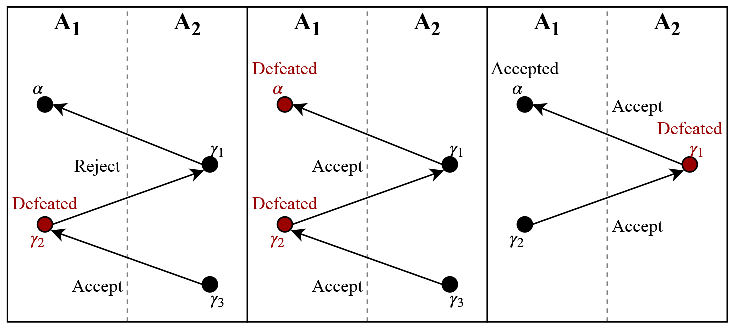
\includegraphics[width=\textwidth]{figs/Resolution.pdf}
    \caption{Once received, an argument is evaluated. If the argument is accepted, the three presented outcomes are possible. The leftmost figure represents the agent $A_{1}$ accepting the argument $\gamma_{3}$ of $A_{2}$: upon the removal of the defeated $\gamma_{2}$, $\gamma_{1}$ is re-evaluated but still rejected and therefore $A_{1}$ will build a new argument against it. The middle figure represents the agent $A_{1}$ accepting $\gamma_{3}$, and upon re-evaluating $\gamma_{1}$ accepts it as well, therefore removing the belief $\alpha$ and left with no other choice than creating a new belief. The rightmost figure represent the agent $A_{2}$ accepting the argument $\gamma_{2}$, removing the defeated argument $\gamma_{1}$ and therefore re-evaluating and then accepting the belief $\alpha$, ending the argumentation.}
    \label{fig:Resolution}
\end{figure}

The argumentation in concept creation takes place in the context of the global argumentation on meanings between the two agents, and therefore follow the same rules. The argumentation is turn by turn based, with each agent taking actions between the moment it receives the token and passes it to the other agent. The argumentation in concept creations involves arguments, and in our model these arguments are messages with specific performatives. The two performatives that are specific to the argumentation in concept creation are:

\begin{itemize}
    \item \textbf{Root-Argument, G-Argument, E-Argument}: the message is simply an argument. The type of argument decides which type of elements are contained in the message.
    \item \textbf{Accept-Argument}: the message does not have any content other than the identifier of the accepted argument.
\end{itemize}

\section{General Structure of Argumentation} 
\label{sec:ArgStruct}

\subsection{Argumentation Goal}
\label{sec:ArgumentationGoal}

When two agents meet, they are prepared to face a situation where they do not understand each other. In order to be ready for argumentation, they both create a copy of their initial contrast set. This copy of their initial contrast set becomes their \emph{current} contrast set. These current contrast sets might be modified later if the agents start an argumentation. The goal of an argumentation is always to make two agents reach mutual intelligibility without changing their contrast sets in a non-monotonic way. While the agents can chose different strategies to reach the mutual intelligibility with this constraint, all strategies have the same final goal and also share similar intermediary goals. 

While Section \ref{sec:AgreeDisagree} presents the characteristic of mutual intelligibility, this section will focus on its achievement from a point where our system of two agents is unable to guarantee it. In this section, we  stated that while the synchronic agreement was probably not initially reached by the agents, the diachronic agreement is initially always found. The diachronic agreement being always initially found is due to the fact that this agreement symbolize the similarity between the initial and the current contrast set. Since the current contrast set is initially a copy of the initial contrast set, there is initially no difference between the two contrast sets and therefore no diachronic disagreement.

\subsection{Argumentation Turns}
\label{sec:ArgTurns}

Our argumentation model is a turn-by-turn model, meaning that only one agent can take take actions at a given time. In order to synchronize the turns, the agents have a \emph{token}. When an agent gets the token, it takes as many actions as it needs to, and then passes the token to the other agent which does the same. The beginning of an argumentation on meaning always starts with the experimenter giving the token to a random agent. The duration which goes from an agent receiving the token and passing it is called the \emph{turn} of this agent.

A turn is always organized following the same structure: first the agent receives the token, then the agent reads its messages, then the agent updates its knowledge according to the new elements received in the messages, then the agent take the actions that are dictated by its current state and its current knowledge, then the agent eventually sends messages to the other agent, then the agent sets its next step, and finally the agent passes the token to the other agent.

\subsection{Argumentation Steps}
\label{sec:ArgSteps}

An argumentation between two agents is always cyclic. At each iteration of the cycle, the agents are closer from the mutual intelligibility than they were during the last iteration -- even if sometime they have more synchronic disagreements than during the last iteration. Each cycle of the argumentation can be divided in steps. In each step, the agents pass by a number of states that determine the agents' actions. Once an agent has taken all the actions that are determined by its current state, it might changes its state and let the other agent take actions. In order to keep track of which agent should take action, the agents have one token. An agent can act only if it has the token. The last action of an agent before an action of the other agent is always passing the token, and if an agent should change its state it always does so as the last action before passing the token.

Each argumentation strategy can be split into four main steps. The first step is to compute some overall pairing relations between concept(s) from different agents. The second step is to infer disagreements from the pairing relations computed during the first step, and to list them. The third step is to pick one disagreement to resolve, and the fourth step is to resolve the disagreement picked during the third step. Once the fourth step is over, the argumentation goes back to the first step in a new iteration of its cycle.

\section{Argumentation Strategies}

The different strategies on argumentation over the meaning diverge by their approach to disagreement identification. The first strategy, called the systematic strategy requires from the agents to exchange all of their intensional definitions when they meet each others. This ensures that two agents using the systematic strategy start their argumentation with knowledge over all the synchronic disagreements between the two agents' initial contrast sets.

The second approach is called the lazy approach. In this approach, the agents are starting their communication with a naming game: an example is presented to them and the agents name this examples. By comparing the sets of signs used by the agent to name the example, the two agents can infer if there is a synchronic disagreement between them.

\section{Resolution of Disagreements}
\label{sec:Resolution}

% Disagreements are resolved when at least one of the two concepts involved in them is removed from its contrast set.
A disagreement can involve a maximum of two concepts. A disagreement might be partially caused by the signs of these two concepts, as it is the case for the lexical disagreements, however all types of disagreements are based on the pairing relation between the two concepts. Since removing one of the concepts from its contrast set removes the pairing relation between them at the same time, removing a concept involved in a disagreement resolves the disagreement.

% The problem can therefore be expressed as replacing the concepts that are causing disagreements by concepts that are not causing disagreements
However, the examples that were covered by a concept that has been removed would not be covered anymore. For this reason, a concept that is removed in order to resolve a disagreement should be replaced by a set of concepts that are not causing synchronic or diachronic disagreements. These new concepts should, as much as they can, cover the examples that were covered by the concepts they are replacing. In this section, we present how our model replaces concepts in disagreements by concepts that are not.

\subsection{Resolving Lexical Disagreements}

\begin{figure}[t]
    \centering
    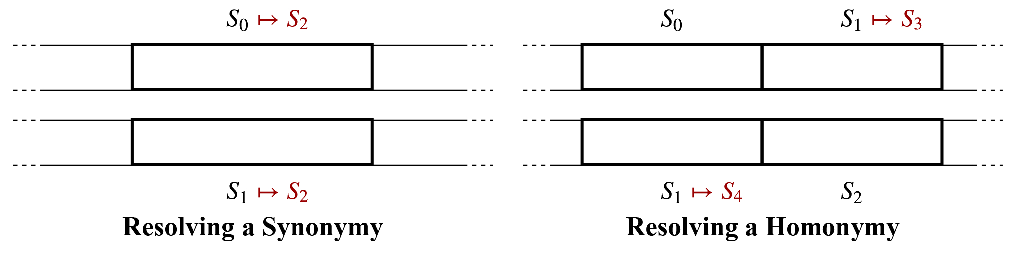
\includegraphics[width=\textwidth]{figs/Lexical.pdf}
    \caption{Caption}
    \label{fig:SolveLexical}
\end{figure}

% The partition is not at fault, the agents just need to change the signs
In the case of a lexical disagreement, the partition made by the two concepts involved in the disagreement are not at fault. The two concepts have a pairing relation of equivalence (homonymy) or are disjoint (synonymy), and the only thing leading them to cause a disagreement is their signs. Therefore, a concept involved in a lexical disagreement is replaced by a concept that share the same intensional and extensional definition, but that has a different sign.

\subsubsection{Resolving Synonymy Disagreements}

% Replace the two synonyms by concepts with a same signs, without touching the other elements
Let $C_{1}$ and $C_{2}$ be two concepts from two agents $A_{1}$ and $A_{2}$, such that their pairing relation in the overall context $U_{O}$ is $C_{i} \equiv_{UO} C_{j}$ and their signs are different: $s(C_{i}) \neq s(C_{j})$. According to Section \ref{sec:SynD}, $C_{i}$ and $C_{j}$ are causing a synonymy disagreement $d_{s}$.
In order to resolve $d_{s}$, each agent $A_{k}$ replaces its concept $C_{k} = \langle s_{k}, I_{k}, E_{k} \rangle$ by a new concept $C'_{k} = \langle s, I_{k}, E_{k} \rangle$. This process is represented in Figure \ref{fig:SolveLexical} (left), where two concepts having different signs $s_{0}$ and $s_{1}$ are replaced by two concepts having the same sign $s_{2}$.
The resulting concepts $C'_{1}$ and $C'_{2}$ are still in a relation of equivalence, since their intensional and extensional definitions remained the same as $C_{1}$ and $C_{2}$, and their signs are now the same. Therefore, according to Section \ref{sec:SynAg}, the pair of concepts $C'_{1}, C'_{2}$ is not causing a disagreement.
As mentioned in Section, \ref{sec:funCreaSign}, the new sign is different from the signs of the overall vocabulary. Therefore, the new concepts cannot cause a homonymy disagreement.

\subsubsection{Resolving Homonymy Disagreements}

% Replace the two homonyms by concepts with different signs, without touching the other elements
Let $C_{1}$ and $C_{2}$ be two concepts from two agents $A_{1}$ and $A_{2}$, such that their pairing relation in the overall context $U_{O}$ is $C_{i} \oslash_{UO} C_{j}$ and they share the same sign: $s(C_{i}) = s(C_{j})$. According to Section \ref{sec:SynD}, $C_{i}$ and $C_{j}$ are causing a homonymy disagreement $d_{s}$.
In order to resolve $d_{h}$, each agent $A_{k}$ replaces its concept $C_{k} = \langle s, I_{k}, E_{k} \rangle$ by a new concept $C'_{k} = \langle s_{k}, I_{k}, E_{k} \rangle$. This process is represented in Figure \ref{fig:SolveLexical} (right), where two concepts having the same sign $s_{1}$are replaced by two concepts having different signs $s_{3}$ and $s_{4}$.
The resulting concepts $C'_{1}$ and $C'_{2}$ are still in a relation of disjunction, since their intensional and extensional definitions remained the same as $C_{1}$ and $C_{2}$, and their signs are now different. Therefore, according to Section \ref{sec:SynAg}, the pair of concepts $C'_{1}, C'_{2}$ is not causing a disagreement.
As mentioned in Section, \ref{sec:funCreaSign}, the two new signs are different from the signs of the overall vocabulary. Therefore, the new concepts cannot cause a synonymy disagreement.

\subsection{Resolving Untranslatable Disagreements}

\begin{figure}[t]
    \centering
    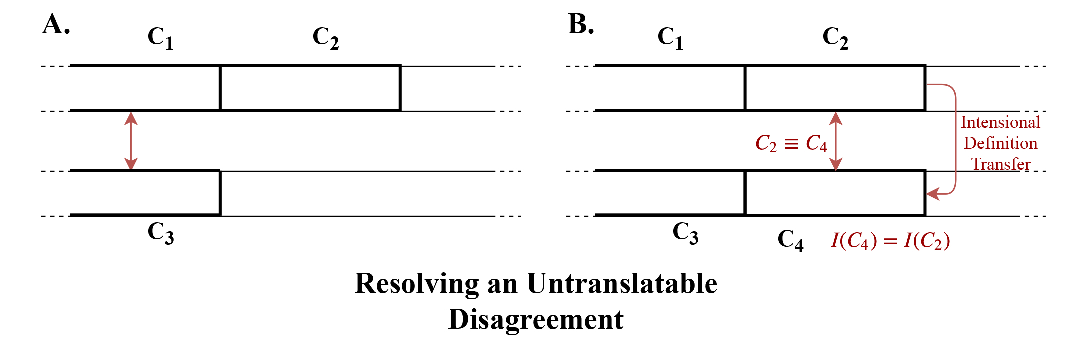
\includegraphics[width=\textwidth]{figs/Untranslatable.pdf}
    \caption{Caption}
    \label{fig:SolveUntrans}
\end{figure}

% One agent needs to create a new concept that is equivalent with the concept of the other agent that does not have an equivalent.
The untranslatable disagreements are a special scenario, as they are not involving two concepts, but one concept and the absence of its equivalent in the other contrast-set. Therefore, an untranslatable disagreement is not resolved by removing a concept but by creating a new one, equivalent to the concept that has no equivalent.
Let $C = \langle s, I, E \rangle$ a concept of the agent $A_{1}$, such that the agent $A_{2}$ has no concept $C'$ in its contrast set such that $C \equiv_{UO} C'$. According to Section \ref{sec:SynD}, this situation results in an untranslatable disagreement $d_{u}$.
In order to resolve $d_{u}$, the agent $A_{2}$ creates a new concept $C' = \langle s, I, Adj(I,U_{2}) \rangle$. Since the two concepts $C$ and $C'$ share their intensional definition -- and thus their adjunct set, they are equivalents according to Definition \ref{def:Relation}.
Now that there exists a concept $C'$ in the contrast-set of $A_{2}$ such that $C \equiv_{UO} C'$, the situation does not cause an untranslatable disagreement anymore.
Since the sign of the concepts $C$ and $C'$ are the same, the two equivalent concepts are not causing a synonymy disagreement.

\subsection{Resolving Self-Disagreements}

\begin{figure}[t]
    \centering
    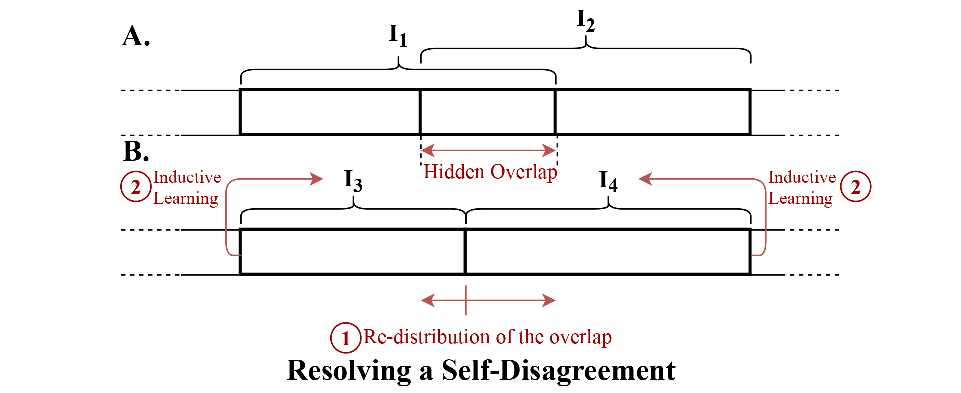
\includegraphics[width=\textwidth]{figs/SelfDisagreement.pdf}
    \caption{Caption}
    \label{fig:SolveSelf}
\end{figure}

% The two concepts are from the same contrast set, only option is that they are in an overall pairing relation of overlap
Let $C_{1}$ and $C_{2}$ two concepts from an agent $A_{1}$ such that $C_{1} \otimes_{UO} C_{2}$. It is important here to note a few things. First of all, since $C_{1}$ and $C_{2}$ belong to a same contrast set, the agent $A_{1}$ cannot see their local pairing relation as $C_{1} \otimes_{U1} C_{2}$, but only as $C_{1} \oslash_{U1} C_{2}$. This means that $A_{1}$ has interacted with another agent $A_{2}$, such that $A_{2}$ has in its local context $U_{2}$ some examples subsumed by both $I(C_{1})$ and $I(C_{2})$.
Moreover, the only pairing relation that can be involved in a self-disagreement is an overlap. Indeed, if $A_{1}$ sees the relation between its two concepts as $C_{1} \oslash_{U1} C_{2}$, this means that there are examples both subsumed by $I(C_{1})$ and not $I(C_{2})$, and examples subsumed by $I(C_{2})$ and not $I(C_{1})$ -- in the local and the overall context. Therefore, the overall pairing relation between $C_{1}$ and $C_{2}$ is either an overlap or a disjunction. Since the signs of the concepts from a same contrast set are all different, the only possible pairing relation causing a disagreement is the overlap. Therefore, a self-disagreement always involves two overlapping concepts.

% Since none of the agent cares to which one of the concept the examples in the overlap should belong to, the agents will use a semantic distance measure that is context independent in order to reassign them
An important specificity of the self-disagreement, is that the examples that are in the overlap of the two concepts have no particular reason to belong to one concept or another. Indeed, the agent $A_{1}$ does not know about these examples, therefore their classification cannot affect its synchronic or diachronic agreement. Moreover, while the agent $A_{2}$ might classify these examples in two or more different concepts, the resulting disagreements should be handled as separate semantic disagreements, not as self-disagreements. For this reason, the two concepts $C_{1}$ and $C_{2}$ should be replaced by a new pair of concepts $C'_{1}, C'_{2}$ such that $C'_{1} \odot_{UO} C'_{2}$ and $Adj(C'_{1},U_{O}) \cup Adj(C'_{2},U_{O}) = Adj(C_{1},U_{O}) \cup Adj(C_{2},U_{O})$.

% Create the new concepts by distributing the examples
The two new concepts will be created through argumentation, one after the other. But the first step for the two agents, is to decide of which sign should be associated to each of the elements from the intersection of $Adj(C_{1},U_{O})$ and $Adj(C_{2},U_{O})$. For now, these examples are associated to both $s(C_{1})$ and $s(C_{2})$, which prevents the creation of a new concept through argumentation. Each agent starts by creating the sets of examples:

\begin{itemize}
    \item $U_{k,C1,\overbar{C2}} = Adj(C_{1},U_{k}) - Adj(C_{2},U_{k})$
    \item $U_{k,C1,C2} = Adj(C_{1},U_{k}) \cap Adj(C_{2},U_{k})$
    \item $U_{k,\overbar{C1},C2} = Adj(C_{2},U_{k}) - Adj(C_{1},U_{k})$
\end{itemize}

% Distances to distribute them
In order to choose, for each example from $U_{1,2,k}$, which sign of $s(C_{1})$ or $s(C_{2})$ is better suited, each agent uses the AU similarity measure. The AU measure quantifies the similarity between an intensional definition $g$ and an example $e$, noted $dAU(g,e)$. Let $I_{1} = \{g_{1,1}, \ldots, g_{1,m}\}$ the intensional definition of $C_{1}$ and $I_{2} = \{g_{2,1}, \ldots, g_{2,n}\}$ the intensional definition of $C_{2}$; For each example $e \in U_{1,2,k}$, $A_{k}$ calculates the average similarities:

\[D_{1} = \frac{1}{|I_{1}|} \times \sum^{m}_{i=1} dAU(g_{1,i},e) \textrm{ and } D_{2} = \frac{1}{|I_{2}|} \times \sum^{n}_{i=1} dAU(g_{2,i},e) \]

% We get a coherent set of associations
Then, $A_{k}$ creates a set of examples $E_{1,k} = \{e \in U_{1,2,k} | D_{1} \geq D_{2} \}$ and a set of examples $E_{2,k} = \{e \in U_{1,2,k} | D_{2} > D_{1} \}$. $A_{k}$ then adds the examples from $U_{1,\overbar{2},k}$ to $E_{1,k}$ and the examples from $U_{\overbar{1},2,k}$ to $E_{2,k}$. Finally, $A_{k}$ associates all the examples of $E_{1,k}$ with $s(C_{1})$ and all the examples of $E_{2,k}$ with $s(C_{2})$. Since the examples of $U_{1,2,k}$ have been re-distributed, the set of associations $E_{1,k} \mapsto s(C_{1}) \cup E_{2,k} \mapsto s(C_{2})$ is coherent. Moreover, since the agents have both access to the intentional definitions $I_{1}$ and $I_{2}$, an example $e$ that is present in both $U_{1,2,1}$ and $U_{1,2,2}$ will have the same associated distances $D_{1}$ and $D_{2}$ independently of the agent that measures them. For this reason, if the example $e$ is put in the set $E_{1,x}$ by $A_{1}$, it will be put in the set $E_{2,x}$ by $A_{2}$ and therefore associated to a same sign. For this reason, the set of associations $E_{1,1} \mapsto s(C_{1}) \cup E_{1,2} \mapsto s(C_{1}) \cup E_{2,1} \mapsto s(C_{2}) \cup E_{2,2} \mapsto s(C_{2})$ is also coherent, authorizing the agents to learn new concepts through argumentation.

% Learning a belief, they arguing
The new concepts $C'_{1}$ and $C'_{2}$ are created through argumentation, sequentially. The agents will start by creating the new concept $C'_{1}$ that will replace $C_{1}$. Following the protocol described in Section \ref{sec:funLeadArg} will lead to the agent $A_{1}$ supervising the creation of $C'_{1}$. $A_{1}$ will therefore create a new belief $\alpha_{1}$ using the set of examples $E_{1,1}$ as a set of positive examples. $A_{2}$ will evaluate this belief using $E_{2,1}$ as the set of positive examples, and eventually argue with $A_{1}$ until it eventually accepts a belief $\alpha' = \langle +, I'_{1}, A_{1} \rangle$. Once the belief is accepted, $A_{1}$ creates the new concept $C'^{1}_{1} = \langle s(C_{1}), I'_{1}, E_{1,1} \rangle$ and replaces $C_{1}^{1}$ with it in its contrast set. Similarly, $A_{2}$ creates a new concept $C'^{2}_{1} = \langle s(C_{1}), I'_{1}, E_{2,1} \rangle$ and replace $C^{2}_{1}$ with it in its hypothesis. Adopting the same strategy for the creation of $C'_{2}$, the agent $A_{1}$ now has a pair of concepts $C'_{1}, C'_{2}$ that are not overlapping in its contrast set.

% They could use other techniques, like distributing every example randomly; making sure that the example has no duplicate in the others concept, but doing so would be an unnecessary cost of examples. Point is: we do not care in which concept they go as long as they stop being in both
Of course, the re-distribution of the examples that are belonging to both the adjunct set $Adj(C_{1},U_{O})$ and the adjunct set $Adj(C_{2},U_{O})$ could be different. Each example $e$ could be randomly assigned to one of the two new concepts $C'_{1}$ and $C'_{2}$, however this would force the agent $A_{k}$ associating $e$ with the sign $s(C_{k})$ to send the association $e \mapsto s(C_{k})$ to the other agent, thus increasing the number of examples exchanged. Without exchanging $e$, the two agents would risk that $A_{-k}$ also has the example $e$ in its contrast-set, and associates it with another sign $s(C_{-k})$. This would result into an non-consistent set of associations on which to build the new intensional definitions upon, which is not possible according to Section \ref{sec:funCreaConA}.

\subsection{Resolving Semantic Disagreements}
\label{sec:ResSemDis}

% Semiotic disagreements are solved through refinement. Concepts involved in semantic disagreements are replaced by their hyponyms
Semiotic disagreements are resolved through the refinement of pre-existing concepts, which means that the concepts involved in a semantic disagreements will either be removed from the contrast set or replaced by a set of co-hyponyms that are partitioning the examples of the concepts involved in the disagreement.

\subsubsection{Resolving Indistinguishable disagreements}

The indistinguishable disagreement is a particular type of example that can only appear if the model admits an error threshold $\tau_{E}$. The notion of error threshold is presented later in Chapter \ref{ErrorManagement}. An error threshold changes the pairing function of our model to neglect non-empty partial sets of comparatively small sizes during the computation of r-triplets. If two newly created concepts $C_{1}$ and $C_{2}$ both have adjunct sets such that $Adj(C_{1}, U_{O}) \geq \tau_{E}$ and $Adj(C_{2}), U_{O} \geq \tau_{E}$ but:

\begin{itemize}
    \item $U_{O,C_{1},C_{2}} < \tau_{E}$ and
    \item $U_{O,\overbar{C_{1}},C_{2}} < \tau_{E}$ and
    \item $U_{O,C_{1},\overbar{C_{2}}} < \tau_{E}$
\end{itemize}

then, the two concepts are considered to be too close from equivalence and one should be removed. The agents resolve the indistinguishable disagreement by removing the concept $C \in \{C_{1}, C_{2}\}$ with the smallest adjunct set $Adj(C, U_{O})$ from the concerned contrast sets. Since $C$ is removed from the argumentation, the disagreement caused by the relation between $C_{1}$ and $C_{2}$ is resolved. This resolution causes a loss in the example coverage of the final contrast set.

\begin{figure}[t]
    \centering
    \includegraphics[width=\textwidth]{figs/Semantic.pdf}
    \caption{Caption}
    \label{fig:SolveSemantic}
\end{figure}

\subsubsection{Resolving Hypo/Hypernymy disagreements}

Let $C_{1} \in S_{1}$ and $C_{2} \in S_{2}$ be two concepts from two agents $A_{1}$ and $A_{2}$, such that their pairing relation in the overall context $U_{O}$ is $C_{1} \odot_{UO} C_{2}$, and let $C_{1}$ be the hypernym of $C_{2}$. According to Section \ref{sec:SynD}, $C_{1}$ and $C_{2}$ are causing a hypo/hypernymy disagreement $d_{h}$.
% Splitting in two co-hyponyms.
In order to resolve $d_{h}$, $A_{1}$ will delete $C_{1}$ from $S_{1}$ and replace it by $C_{3}$, the co-hyponym of $C_{2}$ with regard to $C_{1}$. This process is represented in Figure \ref{fig:SolveSemantic}. The agents use argumentation in order to create $C_{3}$ such that $I(C_{3})$ is best to subsume $Adj(C_{3}, U_{O}) = U_{C1,\overbar{C2},O}$. Since $C_{1}$ is removed from $S_{1}$, the disagreement $d_{h}$ is resolved. However, the overall pairing relations between $C_{3}$ and others concept is unknown except for $C_{2}$.
% In Boolean model, fine because of property 3
If we do not admit an error threshold, we can prove through Property \ref{pp:} that the pairing relation between $C_{3}$ and any other concept is a disjunction, which can only lead to a lexical disagreement (homonymy). If an error threshold is present in the model, the creation of $C_{3}$ can cause further disagreements.

\subsubsection{Resolving Overlap disagreements}

Let $C_{1}$ and $C_{2}$ be two concepts from two agents $A_{1}$ and $A_{2}$, such that their pairing relation in the overall context $U_{O}$ is $C_{1} \otimes_{UO} C_{2}$. According to Section \ref{sec:SynD}, $C_{1}$ and $C_{2}$ are causing an overlap disagreement $d_{o}$.
% Creating a hyponym for the examples in the overlap, resulting in two hypo/hypernym disagreements.
In order to resolve $d_{o}$, $A_{1}$ and $A_{2}$ will both add a concept $C_{3}$ that is the hyponym of both $C_{1}$ and $C_{2}$ to their contrast sets. The agents use argumentation in order to create $C_{3}$ such that $I(C_{3})$ is best to subsume $Adj(C_{3}, U_{O}) = U_{C1,C2,UO}$. Since neither $C_{1}$ nor $C_{2}$ is removed from the agents contrast sets, the disagreement $d_{o}$ is \emph{not} resolved.

However, at least two new disagreements appeared. Since $C_{3}$ is a hyponym of both $C_{1}$ and $C_{2}$, we have $C_{1} \odot_{UO} C_{3}$ and $C_{2} \odot_{UO} C_{3}$. According to Section \ref{sec:SynD}, $C_{1} \odot_{UO} C_{3}$ causes a hypo/hypernymy disagreement $d_{h1}$ and $C_{2} \odot_{UO} C_{3}$ causes a hypo/hypernymy disagreement $d_{h2}$. Since resolving each disagreement $d_{hx}$ involves removing the concept $C_{x}$ as it is a hypernym, the disagreement $d_{o}$ will be resolved upon resolution of $d_{h1}$ and $d_{h2}$.

% In Boolean model, fine because of property 3

 